\section{Results}

\subsection{Monte-Carlo integration}

\subsubsection{Error and accuracy}

\Cref{fig:mc_error} shows the absolute value of the difference between the
calculated value of the integral and the analytical solution with brute force
and importance sampling. N is the number of samples taken. It is worth to notice the sometimes
large differences in error from one run to the next, due to the stochastic nature of
MCI. Still the improvement in accuracy when using importance sampling
is significant especially for larger samples sizes when the standard
deviation is smaller. Yielding an improvement in the error of a factor 10 or
more for sample sizes greater than $10^8$.


\begin{figure}[H]
  \centering
  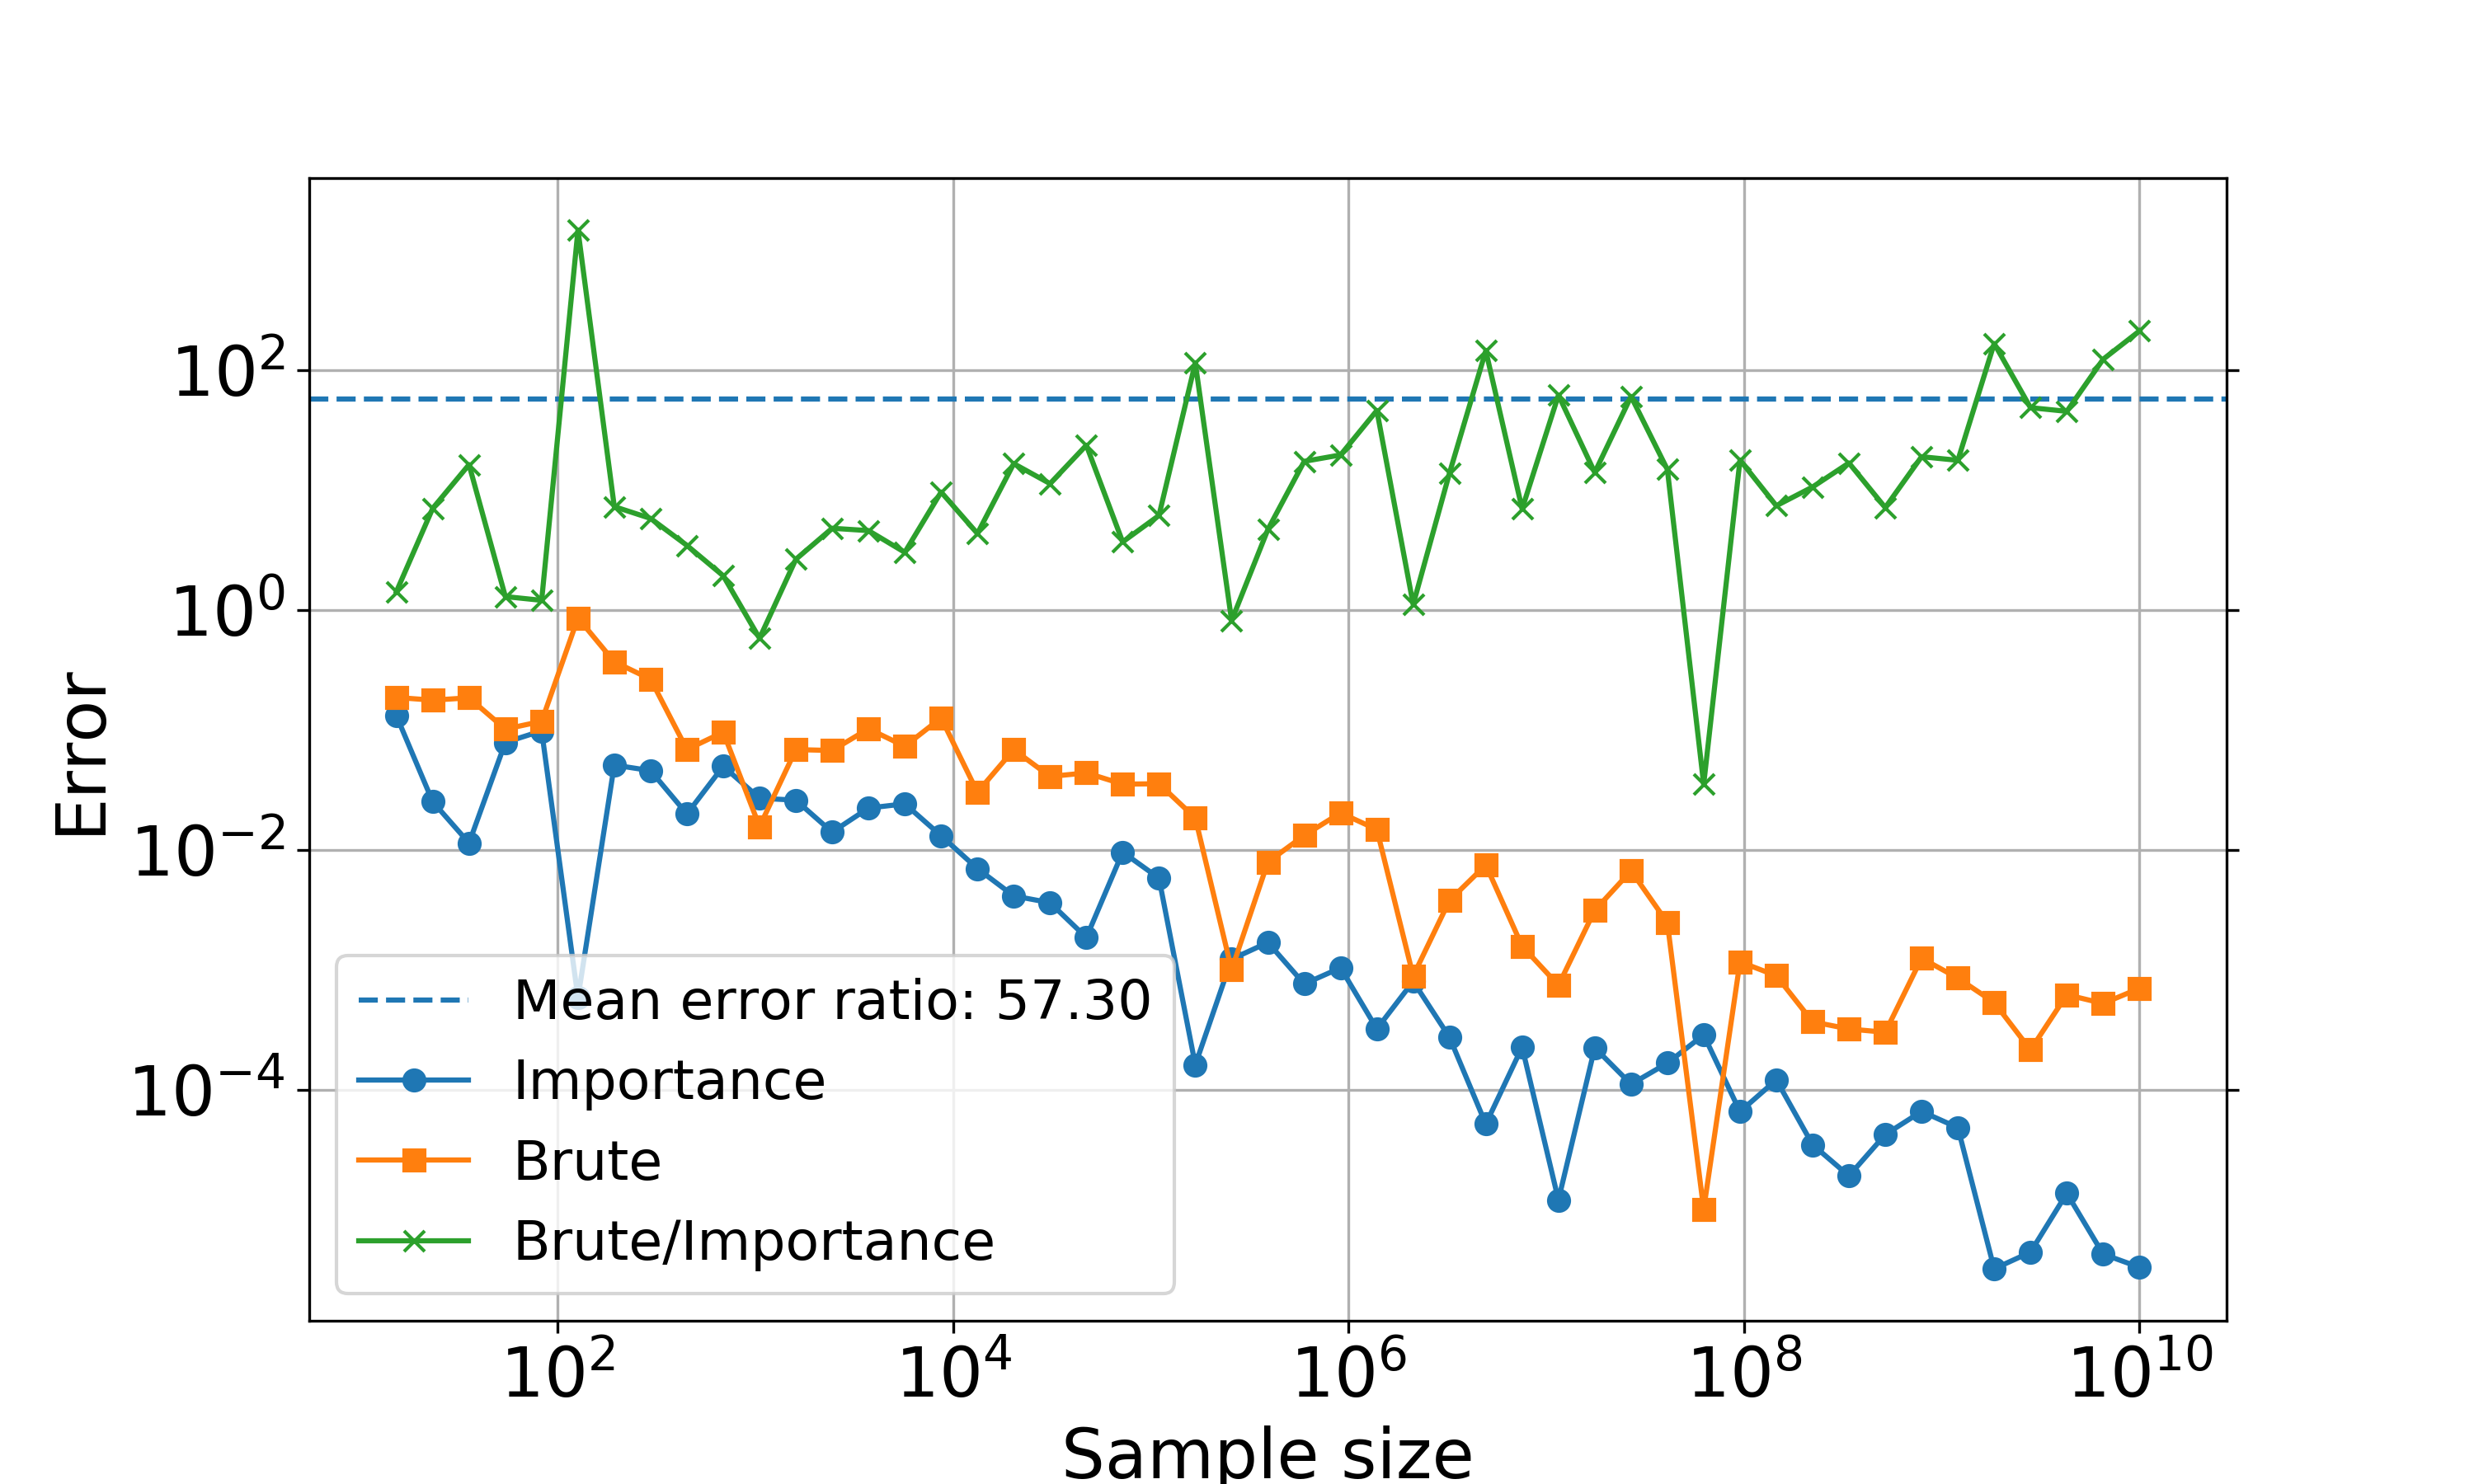
\includegraphics[width=0.8\textwidth]{../figures/mc_error.png}
  \caption{Absolute value of difference between Monte-Carlo results and analytical
  solution using brute force and importance sampling.}

  \label{fig:mc_error}
\end{figure}


\Cref{fig:mc_std_time} shows how the standard deviation evolves with increase in
sample size. For large sample sizes we see that the standard deviation decreases
according to what we would expect from the theoretical expression for the standard
deviation, to reduce the standard deviation by a factor 10 you have increase the
sample size by a factor of 100. 
\Cref{fig:mc_std_time} also show a reduction of the standard deviation by a
factor of 10 for importance sampling MCI compared to brute force MCI.

\begin{figure}[H]
  \centering
  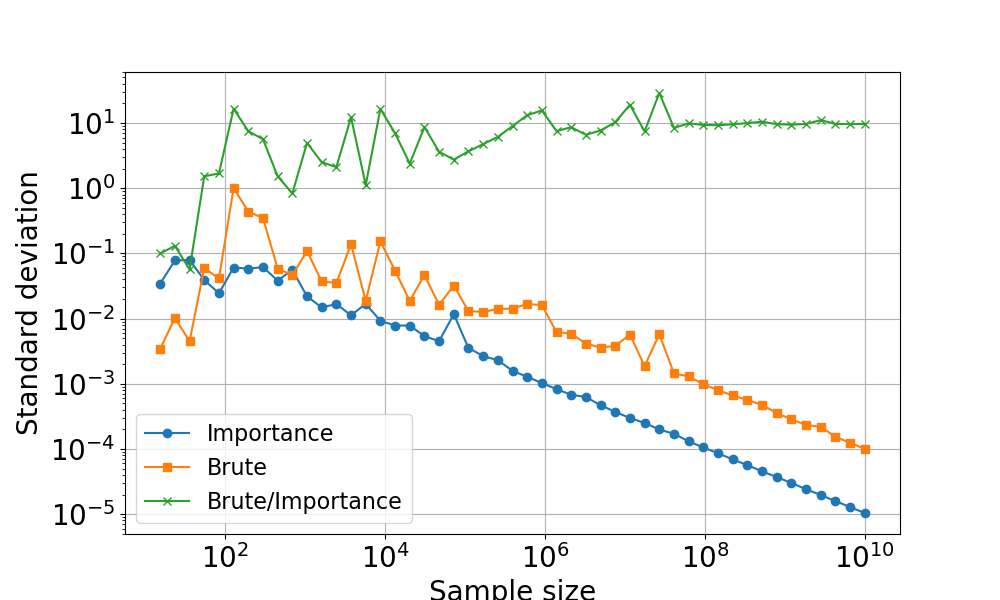
\includegraphics[width=0.8\textwidth]{../figures/mc_std_time.png}
  \caption{Standard deviation versus run time of MCI experiments.}

  \label{fig:mc_std_time}
\end{figure}

\subsubsection{Parallelization}

\Cref{fig:mc_time_ratio} highlight the benefit of parallelization, reducing our
run time by around a factor four. Pretty much would we would expect from the
specifications of our laptop.     

\begin{figure}[H]
  \centering
  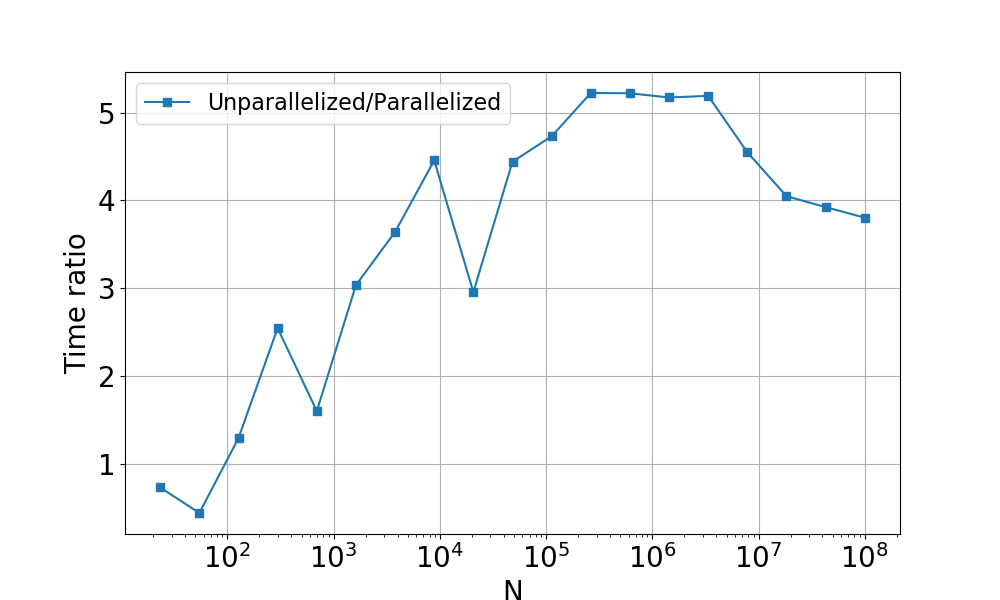
\includegraphics[width=0.8\textwidth]{../figures/mc_time_ratio.png}
  \caption{Run time of MCI using importance sampling. Timing of unparallelized
  version divided by run time of the parallelized version.}

  \label{fig:mc_time_ratio}
\end{figure}


\subsection{Gaussian Quadrature}

The error of the GQ methods \cref{fig:gauss_error} shows that GQLeg gives relatively
low(high) errors when the number of integration points are odd(even). For GQLeg
the error seems to converge around roughly \num{ 5e-3}, and never reaches the
desired error of $10^{-3}$. The GQLag do reach the desired error at N = 14 and 15,
but for higher Ns the error converges to \num{2e-3}, and does not show the oscillatory
nature of the GQLeg.

\begin{figure}[H]
  \centering
  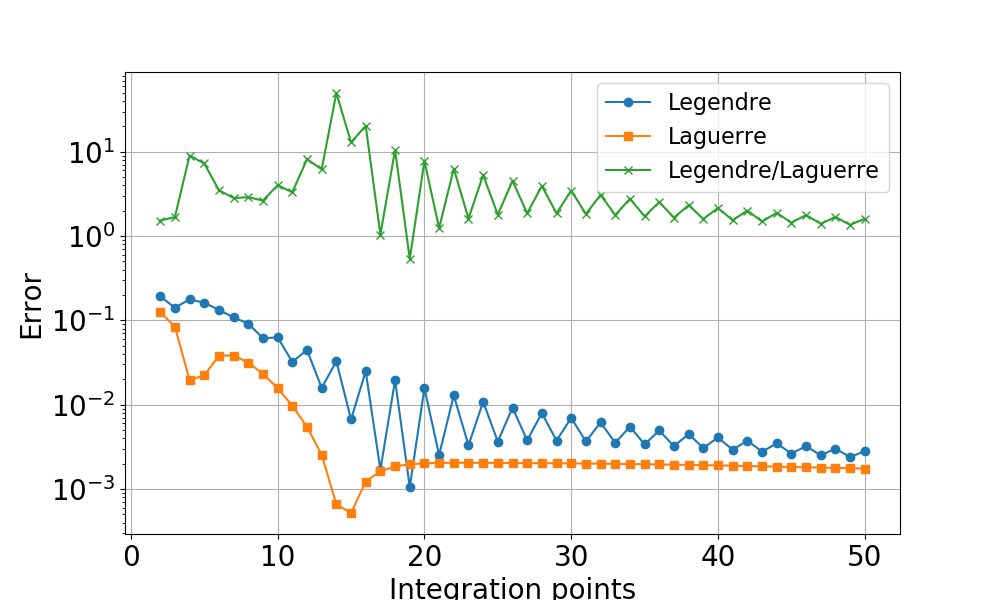
\includegraphics[width=0.8\textwidth]{../figures/gauss_error.png}
  \caption{Absolute value of difference between gaussian quadrature results and analytical
  solution using Legendre and Laguerre polynomials..}

  \label{fig:gauss_error}
\end{figure}


\subsection{Comparison of Gaussian Quadrature and Monte-Carlo Integration}

To clarify whether running Gaussian Quadrature or Monte-Carlo Integration would
give the best results for a given run time we made error-runtime plots for all
of the methods we have used \cref{fig:time_compare}. For MCI low values of runtime
corresponds to few samples, and for GQ it corresponds to a small number of integration points.
For the shortest runtimes the results of MCI were a bit all over the place, but
looking at longer runtimes we see a clear trend of the error decreasing, especially
for the importance sampling.


\begin{figure}[H]
  \centering
  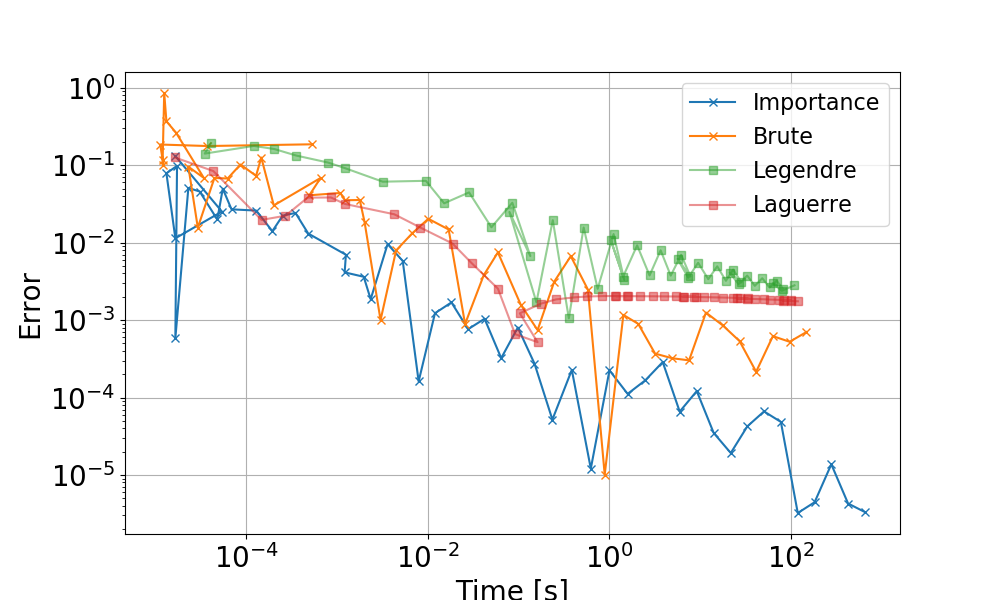
\includegraphics[width=0.8\textwidth]{../figures/time_compare.png}
  \caption{Absolute values of the error as a function of time for all methods we
  used to approximate the integral.}

  \label{fig:time_compare}
\end{figure}
